\documentclass[10pt,oneside,swedish]{lips-no_customer}

%\usepackage[square]{natbib}\bibliographystyle{plainnat}\setcitestyle{numbers}
\usepackage[round]{natbib}\bibliographystyle{plainnat}
\usepackage{parskip}

\usepackage{afterpage}
\graphicspath{{./figures/}}

% Configure the document
\title{Designspecifikation}
\author{Yc.4}
\date{2019-10-09}
\version{0.3}

\reviewed{}{}
\approved{}{}

\projecttitle{Bilbana}

\groupname{Yc.4}
\groupemail{team_yc4@liuonline.onmicrosoft.com}
\groupwww{https://www.fs.isy.liu.se/Edu/Courses/TFYY51/}

\coursecode{TFYY51}
\coursename{Ingenjörsprojekt}

\orderer{Erik Frisk, Linköpings universitet}
\ordererphone{+46(0)13-285714}
\ordereremail{erik.frisk@liu.se}

% \customer{Kund, Företag X}
% \customerphone{+46 xxxxxx}
% \customeremail{customer@companyx.com}

\courseresponsible{Urban Forsberg}
\courseresponsiblephone{+46(0)13-281350}
\courseresponsibleemail{urban.frsberg@liu.se}

\supervisor{Viktor Leek}
\supervisorphone{+46(0)13-284493}
\supervisoremail{viktor.leek@liu.se}

\smalllogo{logo} % Page header logo, filename
\biglogo{logo} % Front page logo, filename

\cfoot{\thepage}
\begin{document}
\maketitle

\cleardoublepage
\makeprojectid

\cleardoublepage
\tableofcontents

\cleardoublepage
\section*{Dokumenthistorik}
\begin{tabular}{p{.06\textwidth}|p{.1\textwidth}|p{.45\textwidth}|p{.13\textwidth}|p{.13\textwidth}} 
  \multicolumn{1}{c}{\bfseries Version} & 
  \multicolumn{1}{|c}{\bfseries Datum} & 
  \multicolumn{1}{|c}{\bfseries Utförda förändringar} & 
  \multicolumn{1}{|c}{\bfseries Utförda av} & 
  \multicolumn{1}{|c}{\bfseries Granskad}\\
  \hline
  \hline
  0.1 & 2019-10-07 & Första utkast & Gustav & \\\hline
  0.2 & 2019-10-08 & Andra utkast & Alla & \\\hline
  0.3 & 2019-10-09 & Tredje utkast, mer detaljerat & Alla & \\\hline
  \hline
\end{tabular}

\cleardoublepage
\pagenumbering{arabic}\cfoot{\thepage}

\section{Syfte och mål}

Syftet med projektet är att konstruera ett system som kör bilar att runt en
bilbana. Till bilbanan finns det 9 ``givare'' som när de passeras skickar en
signal. Med hjälp av tidsskillnaden mellan signalerna kan man räkna ut hur lång
tid det tog för en bil att åka mellan två givar. Bilbanan är även kopplad till
en dator där det finns möjlighet att justera bilarnas gaspådrag med en
spänningstillförsel. Med hjälp av denna information ska ett system skapas som
kör en eller två bilar runt bilbanan på en inställbar varvtid mellan 12 och 15
sekunder, samt gör att bilarna åker i mål så nära varandra i tiden som möjligt.

\section{Delsystem}

Systemet är indelat i två olika delsystem. Dessa system kommer köras
sekvensiellt, alltså det ena efter det andra. Det första systemet kontrollerar
själva bilkörningen medan det andra systemet kontrollerar displayen. Se
figur~\ref{fig:system_diagram} för ett processchema.

\begin{figure}
  \centering
  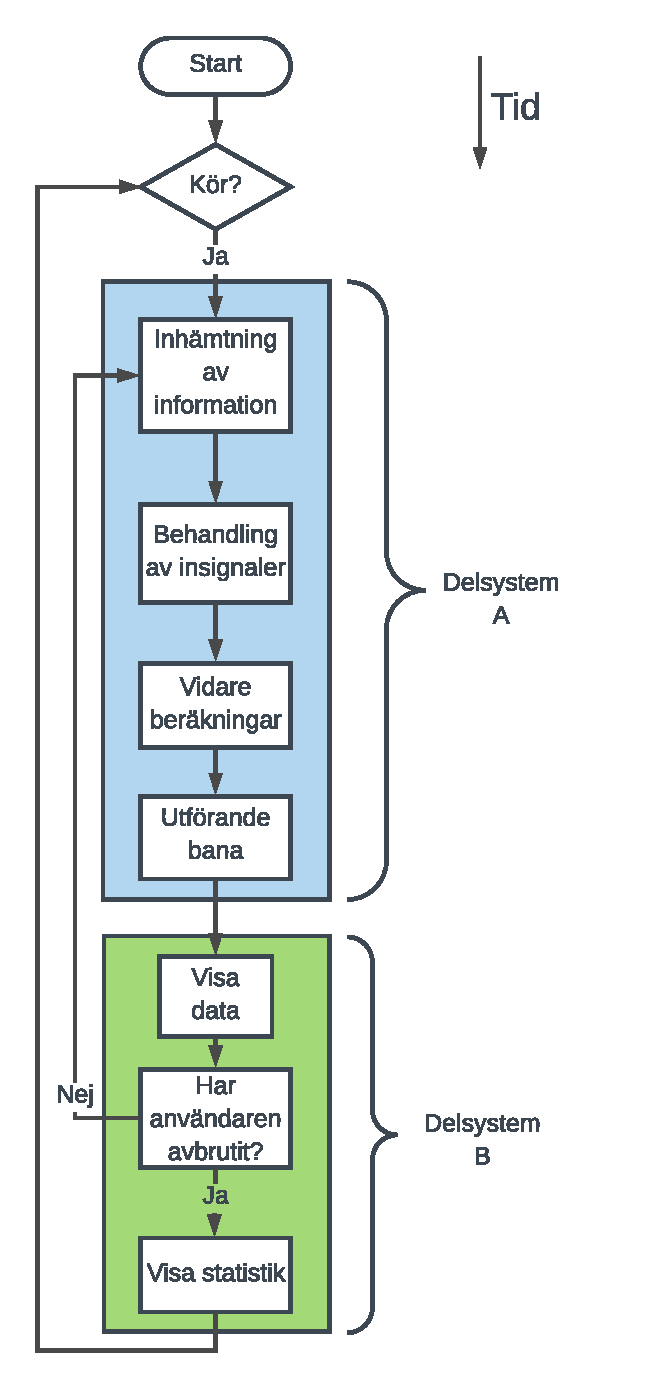
\includegraphics[width=\linewidth,height=0.9\textheight,keepaspectratio]{figures/Processchema.pdf}
  \caption{Processchema över systemets helhet.}%
  \label{fig:system_diagram}
\end{figure}

  \subsection{Delsystem A: Bana}
  
  Delsystem A är indelat i tre övergripande delar. I del A.1 hämtas all
  tillgänglig information in, i del A.2a görs beräkningar utifrån tillgänglig
  data, i del A.2b görs vidare beräkningar (alltså beräkningar som inte baseras
  direkt på den tillgängliga informationen), och i del A.3 utförs de ändringar
  som programmet bedömer är nödvändiga för att klara den valda varvtiden. 

    \subsubsection{Inhämtning av information}

    Information som finns tillgänglig är kraftigt begränsad. I praktiken kommer
    programmet endast fråga om någon av bilarna passerat en givare sedan
    programmet frågade förra gången.

    \subsubsection{Primära beräkningar}

    De primära beräkningarna är de beräkningar som beror direkt på tillgänglig
    information. Eftersom indatan enbart består av bilens position är bilens
    hastighet genom det förra segmentet den enda informationen som direkt beror
    på indata.

    \subsubsection{Sekundära beräkningar}
    
    Den första beräkningen som görs är bilens nuvarande position. Detta görs med
    hjälp av en intern bild av banan och vetskapen om vilken hastighet bilen
    önskas ha. Sedan räknas den position som bäst gör att bilen klarar den satta
    varvtiden ut. För att räkna ut den beaktas enbart den nuvarande tiden och
    (om gemensam målgång är aktiverat) positionen av den andra bilen. Steget
    efter är att räkna ut den mest rimliga optimala situationen som beaktar hur
    lång tid det är kvar på det nuvarande varvet. I början av varvet görs alltså
    inte lika drastiska hastighetsändringar som mot slutet.

    Det sista som händer är när informationen om bilens och banans skick används
    för att räkna ut vilket spänningspådrag som krävs för att få bilen att nå
    den hastighet och position som krävs.

    \subsubsection{Utförande}

    I utförandet skickas det nya spänningspådraget till banorna. 
	

    \subsubsection{Funktioner i delsystem A} \label{sec:system_a_funcs}
    I figur~\ref{fig:flow_diagram}  visas flödet av de funktioner som sker i delsystem A under en cykel.
    Här listas namn på funktionerna och deras funktion:
    \begin{itemize}
	\item old\textunderscore u: old u är lagring av data från bilens spänning. Denna databas kommer lagra information om tidigare cyklar, varv och tidigare lopp. Databasen kommer vara en egen separat funktion så att det blir lätt att referera till databasen.
	\item old\textunderscore v: old v är lagringen av data från bilens hastighet mellan segment, varv, tidigare lopp och detta lagras i databasen som är en egen funktion som vi kommer att referera till. 
	\item old\textunderscore position: Lagring av gammal data för bilens placering. Från denna databas kan andra funktioner få information om var bilen var förra cykeln, var bilen var för ett varv sedan m.m.
      \item indata: Ger data när bilen passerar en givare.
      \item car\textunderscore constant: Programmets sätt att anpassa sig efter olika bilars egenskaper. Justeras vid varje ny indata.
      \item position: Position, programmet räknar ut vart på banan bilen befinner sig genom att hämta senaste positionen old position och sedan addera sträckan bilen har färdats sedan dess senaste värde. Sträckan som bilen har färdats kan räknas ut genom S=V\textasteriskcentered T, där v = old\textunderscore v och (delta)t = tidskillnaden mellan senaste cykel. Om ny indata finns denna cykel så är positionen känd och denna data används i stället för att utgå igrån gammal.
      \item clock: Hur länge bilen har varit i det nuvarande segmentet och varvet.

      \item car\textunderscore position\textunderscore dif: Endast aktiv om gemensam målgång aktiverad. Jämför bilarnas position med varandra. Funktionen utgår ifrån respektive bils placering (från old position) och hastighet (från old v) 
och ger ett värde på placeringsskillnaden för en viss hastighet. Detta kommer
sedan användas för att sätta bilarnas nya hastighet. Värdet blir stort om skillnaden i placering är stor men justeras också efter hastigeten. Dvs om bilarna ligger långt ifrån varandra men åker ganska fort kommer inte värdet bli lika stort som om bilarna legat lika långt ifrån varandra men haft lägre hastighet. Värdet är positivt om bil 1 ligger före bil 2 och negativt om bil 2 ligger före bil 1. På så sätt kan nästa funktion avgöra vilken bil som ligger först.
Värdet används sedan för att beräkna nästa hastighet (new v) som kommer ökas eller minskas för att få bilarna att köra ikapp varandra. 

      \item target: Den varvtid som manuellt har satts innan programet startade.
      \item target dif:Den differensen mellan den önskade tiden och positionen relativt till den faktiska tiden och positionen. Görs genom att subtrahera de önskade värdena med de faktiska värdena.  
      \item agressivness:Justerar hur stora ändringar som görs på new\textunderscorev, vid start av ett nytt varv finns det mycket tid kvar att justera. Följden av detta är att new\textunderscorev kan ändras lite i taget istället för att göra stora förändringar. Angresivness räknas ut via; clock,  vilken tid på varvet bilen befinner sig, Target \textunderscore dif,  hur långt ifrån måltiden befinner sig bilen och om gemensam målgång är aktiv tar agresivness även hänsyn till car\textunderscore position \textunderscore dif,  hur långt är avståndet mellan de två bilarna. 
      \item u\textunderscore constant\textunderscore map: Är en kartläggning över banan och de spänningsnivåer som behöver sättas så att spänningen blir jämn. Detta eftersom att spänningstillförseln beter sig olika för olika delar av banan. Kartläggningen kommer bygga på det register med inlagrad data som tagits fram genom tester.
      \item target\textunderscore dif: Bilens position relativt till var den borde vara vid den nuvarande tiden.
      \item track\textunderscore u\textunderscore constant: Detta ät det förbestämda spänningsvärdet för ett visst subsegment på banan. Värdet tas fram manuellt genom prövning och lagras i u \textunderscore constant \textunderscore map. Ur position tar track \textunderscore u \textunderscore constant fram rätt spänningsvärde. 
      \item speed\textunderscore map: En ``karta'' över hur fort man kan köra i olika delar av banan.n.
      \item speed\textunderscore constant: Den förbestämda hastigheten för nuvarande subsegment. Hastigheten tas fram manuellt genom prövning och lagras i speed \textunderscore map. Ur position tar speed \textunderscore constant fram rätt hastighet. 
      \item new\textunderscore v: Den nya hastigheten som ska sättas.
      \item new\textunderscore u: Den spänning som skickas till bilen.

    \end{itemize}

    \begin{figure}
      \centering
      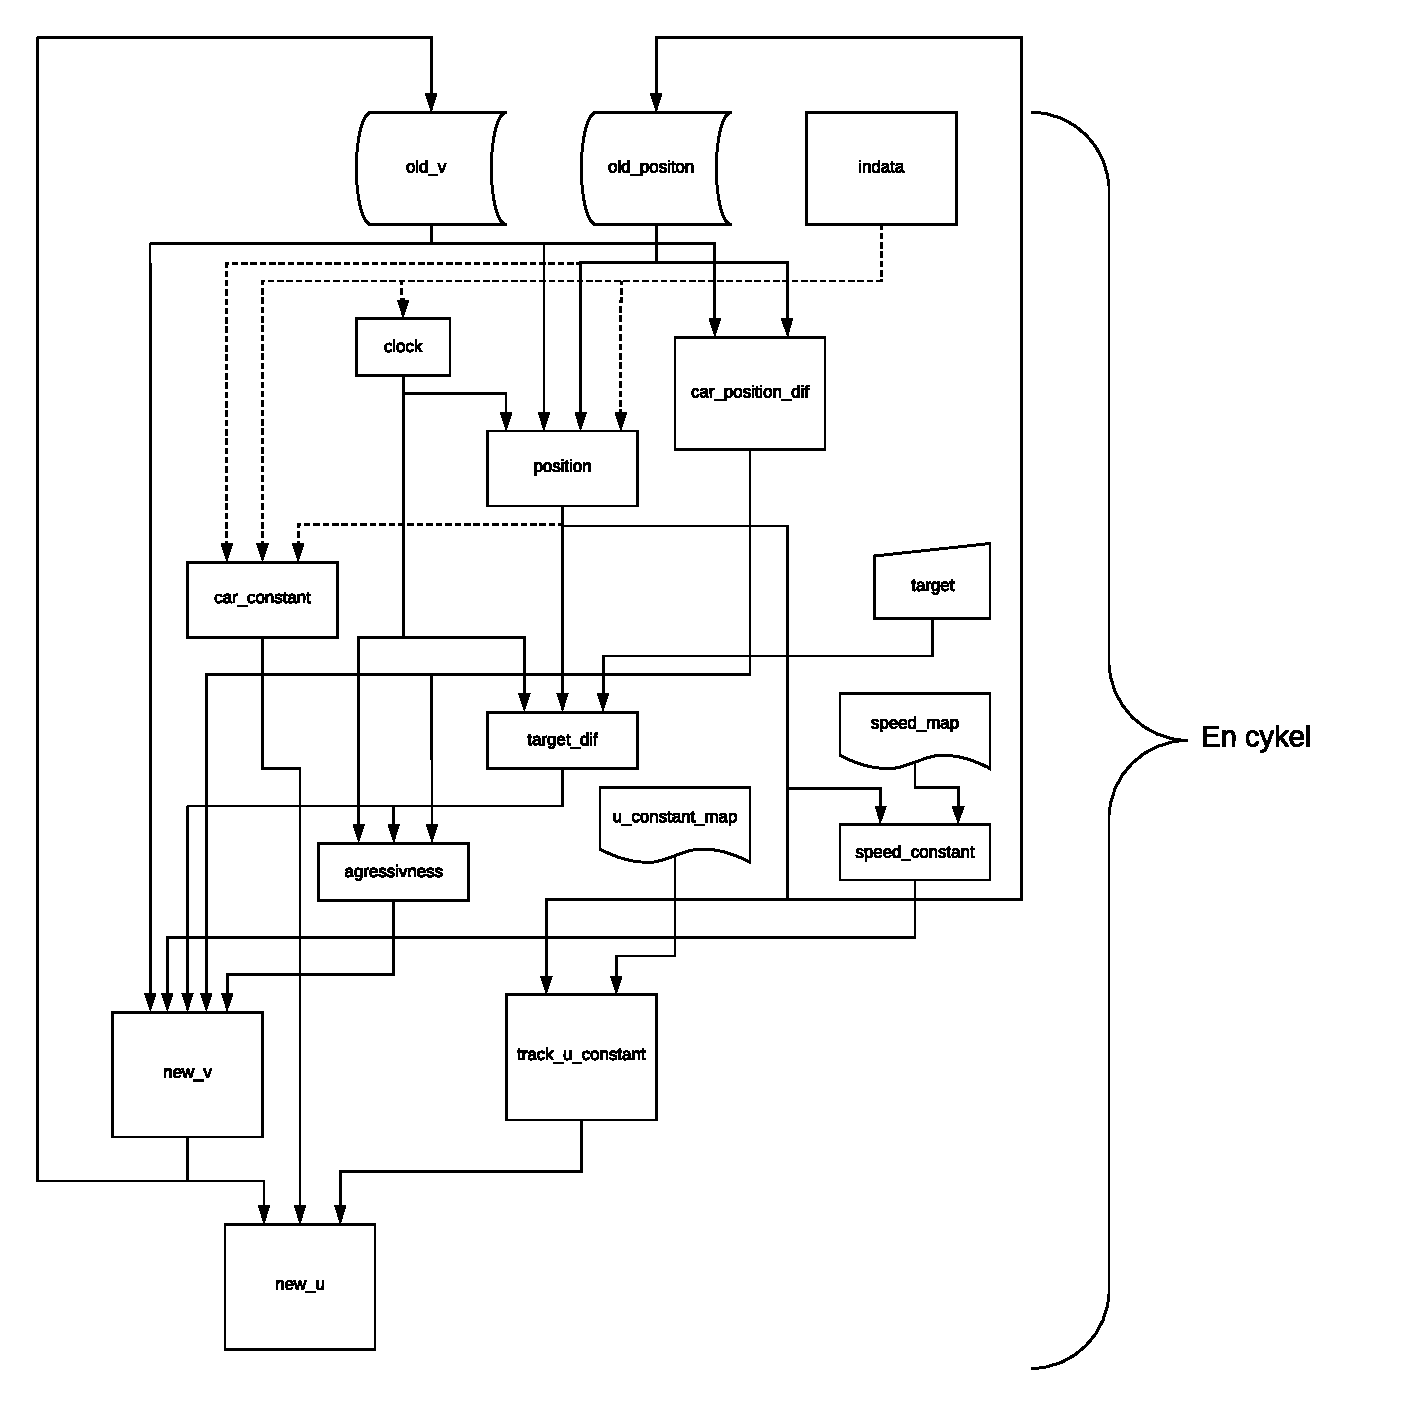
\includegraphics[width=\linewidth]{figures/flow.pdf}
      \caption{Funktionsflödet i delsystem A.}%
      \label{fig:flow_diagram}
    \end{figure}

  \subsection{Delsystem B: Display}

  Displayen ter sig enklare än delsystem A. Under körning ska, om ett nytt varv
  påbörjats, den senaste varvtiden och varvnumret skickas till displayen. Om
  stopp-knappen har tryckts ned ska systemet hoppa till resultat-skärmen och om
  inte så ska det fortsätta.


\section{Display}

När programmet startas visar displayen möjligheten att välja aktiv bana, om
gemensam målgång ska vara aktiverad, vilken varvtid bilarna ska hålla och
eventuellt hur många varv bilarna ska köra runt banan (exkluderat de fem
kalibreringsvarven). Se figur~\ref{fig:disp:before}.

Under körning ska displayen för varje bil visa den förra varvtiden, hur många
varv bilen kört, nuvarande hastighet och pålagd spänning. Användaren kan också
trycka på en knapp för att avbryta körningen. Se figur~\ref{fig:disp:during}. I
mån av tid ska displayen även visa en karta över banan och var systemet tror
att bilarna befinner sig.

Efter körningen är avklarad ska displayen visa olika grafer. Enligt
kravspecifikationen ska varvtid per varv och snitthastigheten för varje segment
visas enligt figur~\ref{fig:disp:after}. I mån av tid ska endast en graf åt
gången visas på skärmen och användaren ska kunna välja vilken graf som ska
visas med hjälp av tryckbara knappar längst upp på skärmen.

\begin{figure}
  \centering
  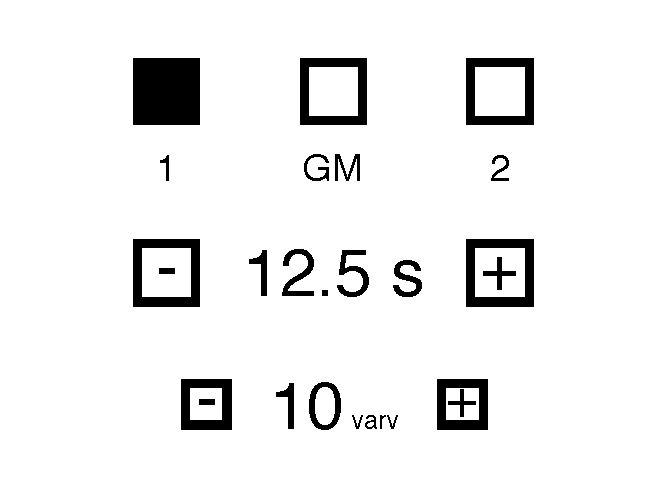
\includegraphics{figures/innan}
  \caption{Displayens utseende vid val av körinställningar.}
  \label{fig:disp:before}
\end{figure}
\begin{figure}
  \centering
  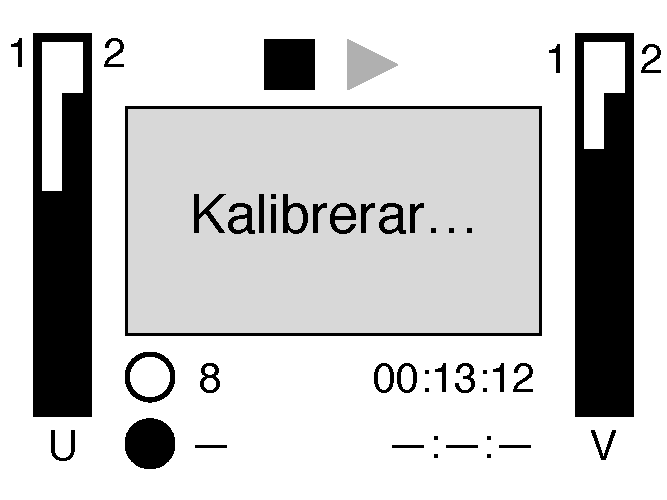
\includegraphics{figures/under}
  \caption{Displayens utseende under körning.}
  \label{fig:disp:during}
\end{figure}
\begin{figure}
  \centering
  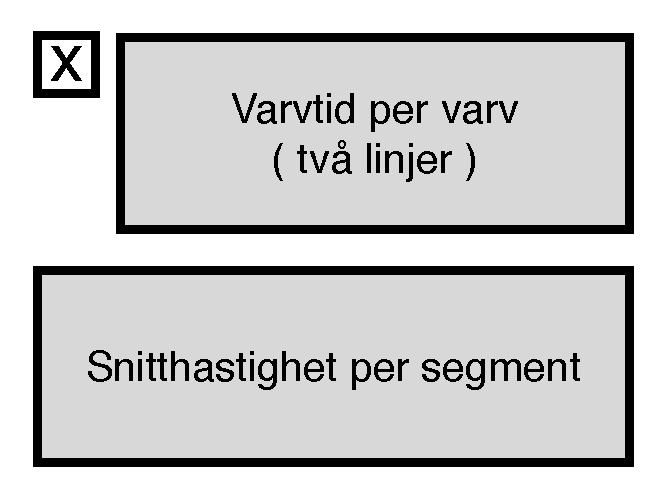
\includegraphics{figures/efter}
  \caption{Displayens utseende när körning är avklarad.}
  \label{fig:disp:after}
\end{figure}

\section{Hantering av händelser}


\subsection{Start}
Innan målgivaren hittar vi ett läge där alla bilar är körbara och inte fastnar. Till första givaren behåller bilen den spänning den behövde för att börja rulla och vi kan därefter veta hur lång tid det tagit mellan start och och första givaren. Med det kan vi räkna ut vilket vilken konstant (k) som bilen behöver. 

\subsection{Avåkning}
Programmet ska detektera att en bil har åkt av banan inom 10 sekunder. Detta
ska göras genom att felvarna, avbryta programmet och skriva ut detta på
displayen om programmet inte registrerar en ny givare inom dessa tio sekunder.


Enligt krav 3 i kravspecifikationen ska programmet kunna hantera missade givare
och fortsätta köra som normalt. Med den metod som kommer användas blir detta inte ett problem.
Givarna kommer endast att användas för att justera programmets uppfattnting om bilarnas position, 
själva positionen ska beräknas på annat sätt.  Programmet ska detektera detta
fel genom att  se om en givare passeras när förväntat. Om den inte gör det och nästa
passering av givare sker när förväntat kommer programmet
identifiera den tidigare tidsfördröjningen som en missad givare.

\subsection{Missade givare}

Enligt krav 3 i kravspecifikationen ska programmet kunna hantera missade givare och fortsätta köra som normalt. Som vi har tänkt att använda oss av givarna så ska inte bilarna ändra sin körning vid ett sådant utfall. Då vi tänkt att använda givarna som en referens och inte justering av bilarnas körning så kommer en missad givare ge ett fel på referens. Programmet ska detektera detta fel genom att med dess interna lagring av data se om det nästa förväntade tidspassering stämmer överrens med nästa givare detektering. Om nästa förväntade tid stämmer överrens med en givares detektering kommer programmet identifiera den tidigare tidsfördröjningen som en missad givare.

Enligt kravspecifikationens punkt 12 ska det vara möjligt att välja om en bana
ska köras manuellt eller autonomt. Det ska alltså gå att köra ena banan
manuellt medan den andra styrs av programmet. Detta styrs via displayen vid
uppstart.


\subsection{Manuell körning}
Enligt kravspecifikationens punkt 12 ska de två olika banorna delas upp så att ena banan styrs autonomt och den andra manuellt. 
Den manuella delen ska bli hjälpt av programmet för att underläta körning vid händelse av driftfall samt uppvärmning av banan.
Detta ska uppnås genom att jämföra vilken hastighet bilen erhåller i ett visst segment styrt av vilken spänningspåläggning som verkar på bilen.
Sedan ska programmet  jämföra hastigheten med en tidigare föreslagen hastighet och sedan modifiera en konstant för att matcha det önskade värdet.

Programmet ska detektera att en bil har åkt av banan inom 10 sekunder. Detta ska göras genom att felvarna, avbryta programmet och skriva ut detta på displayen om programmet inte registrerar en ny givare inom dessa tio sekunder.


\end{document}

%%% Local Variables:
%%% mode: latex
%%% TeX-master: t
%%% End:
